The notation adopted here is that used in~\cite{siegel-howell-3} and in~\cite{catalog}. The configuration factor from a differential area element $dA_1$ to a second element $dA_2$ is denoted by $dF_{d1-d2}$. In general, such a factor is given by 
\begin{equation}
dF_{d1-d2}=\frac{\cos \theta_1 \, \cos \theta_2}{\pi S_{1-2}^2}\,dA_2
\end{equation}
where the quantities on the right-hand-side are shown in Fig.~\ref{fig:in-fi(1)}
\begin{figure}[htbp]
\begin{center}
 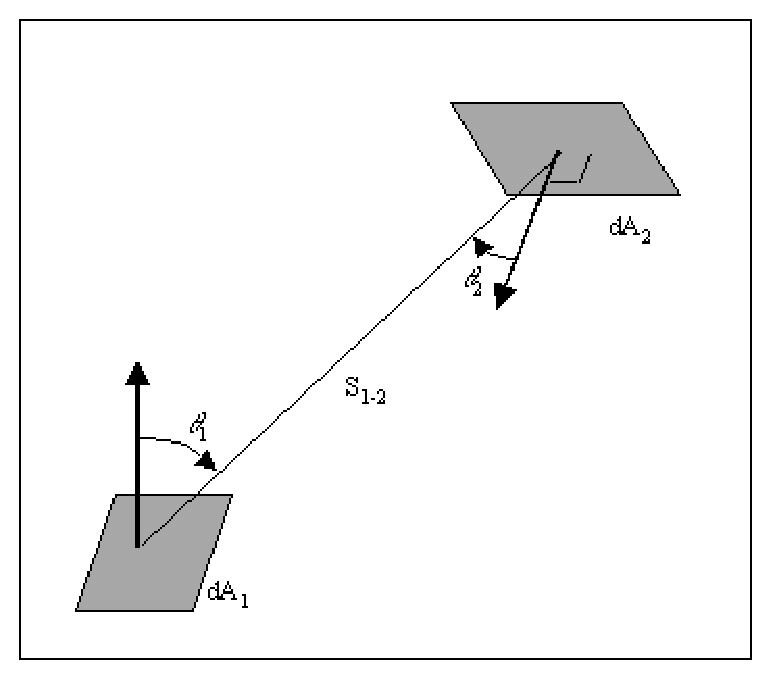
\includegraphics[width=8cm]{Sec_SiteInfra/Cryotraps/in-fi(1).pdf}
			\caption{Defining geometry for configuration factor (from \cite{catalog})}
\label{fig:in-fi(1)}
\end{center}
\end{figure}

For the case of A1 and A2 both finite, the configuration factor is 
\begin{equation}
F_{1-2 } = \frac{1}{A_1}\int_{A_1}\int_{A_2}\frac{\cos \theta_1 \, \cos \theta_2}{\pi S_{1-2}^2}\,dA_2\,dA_1
\end{equation}
leading to the reciprocity relation 
\begin{equation}
A_1 F_{1-2} = A_2 F_{2-1}
\end{equation}

For each section at fixed temperature we need to calculate the geometric factor of the interior surface of circular cylinder of radius $R$ to a disk of radius $r$ where $r < R$. The disk is perpendicular to axis of cylinder, and the axis of the cylinder passes through center of disk (see Fig.~\ref{fig:C-82fig_n})~\cite{siegel-howell-4, buschman_1961}. 
\begin{figure}[htbp]
\begin{center}
 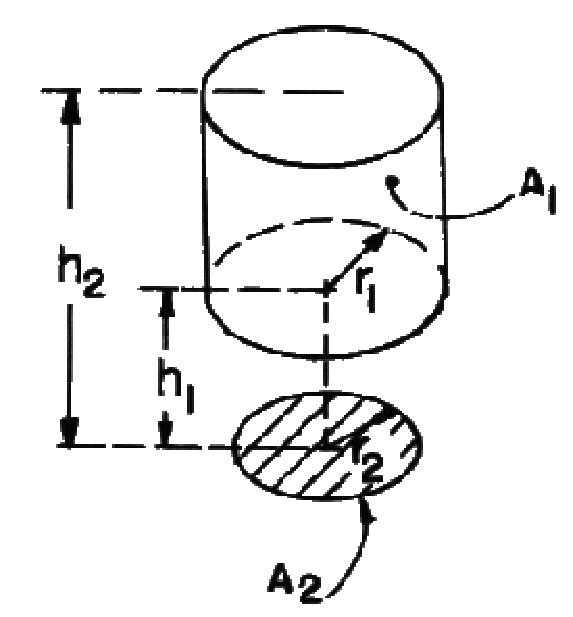
\includegraphics[width=6cm]{Sec_SiteInfra/Cryotraps/C-82fig_n.pdf}
			\caption{Defining symbols in eq.\ref{eq:definitions} and eq.\ref{eq:configuration} (from \cite{catalog})}
\label{fig:C-82fig_n}
\end{center}
\end{figure}

With the definitions:
\begin{eqnarray}
\label{eq:definitions}
R & = & \frac{r_1}{r_2} \\
H_1 & = & \frac{h_1}{r_2} \\
H_2 & = & \frac{h_2}{r_2} \\
X & = & H^2 + R^2 + 1
\end{eqnarray}
the equation is:
\begin{equation}
\label{eq:configuration}
F_{1-2} = \frac{1}{4R(H_2-H_1)}\left[ (X_1-X_2) - (X_1^2 -4R^2)^{1/2} + (X_2^2 -4R^2)^{1/2} \right]
\end{equation}
